\chapter{Sučelja web aplikacije}
\noindent \textbf{Sučelja anonimnog korisnika}\\
\noindent Na slici 4.1. možemo vidjeti sučelje koje se prikazuje pri pokretanju aplikacije. Svakom anonimnom korisniku su u navigacijskoj traci omogućene opcije za povratak na početnu stranicu, prijavu u aplikaciju, pristup stranici s informacijama i pristup kontaktnoj formi. Klikom na gumb "Započnimo" korisnika se također preusmjerava na stranicu za prijavu
\begin{figure}[H]
					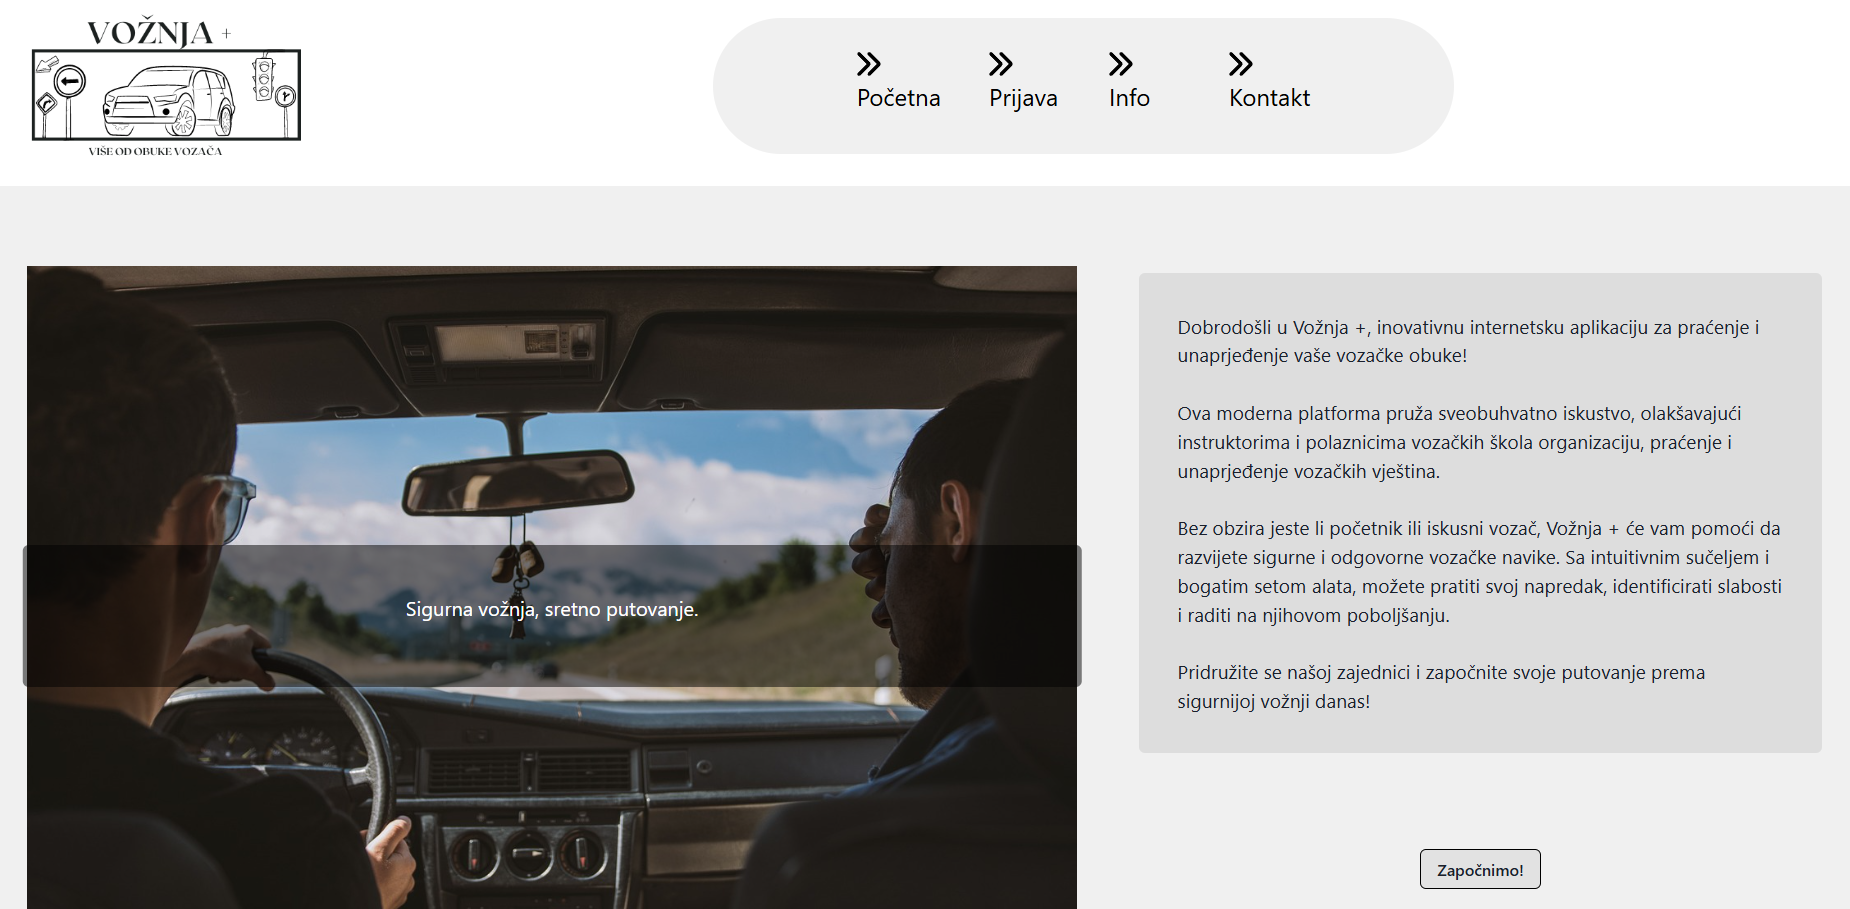
\includegraphics[width=\textwidth]{slike/anoniman1.png} 
					\centering
					\caption{Početna stranica}
					\label{fig:promjene}
				\end{figure}

\noindent Da bi se korisnik prijavio u sustav, u navigacijskoj traci odabire opciju za prijavu. Sučelje koje se prikazuje može se vidjeti na slici 4.2.

\begin{figure}[H]
					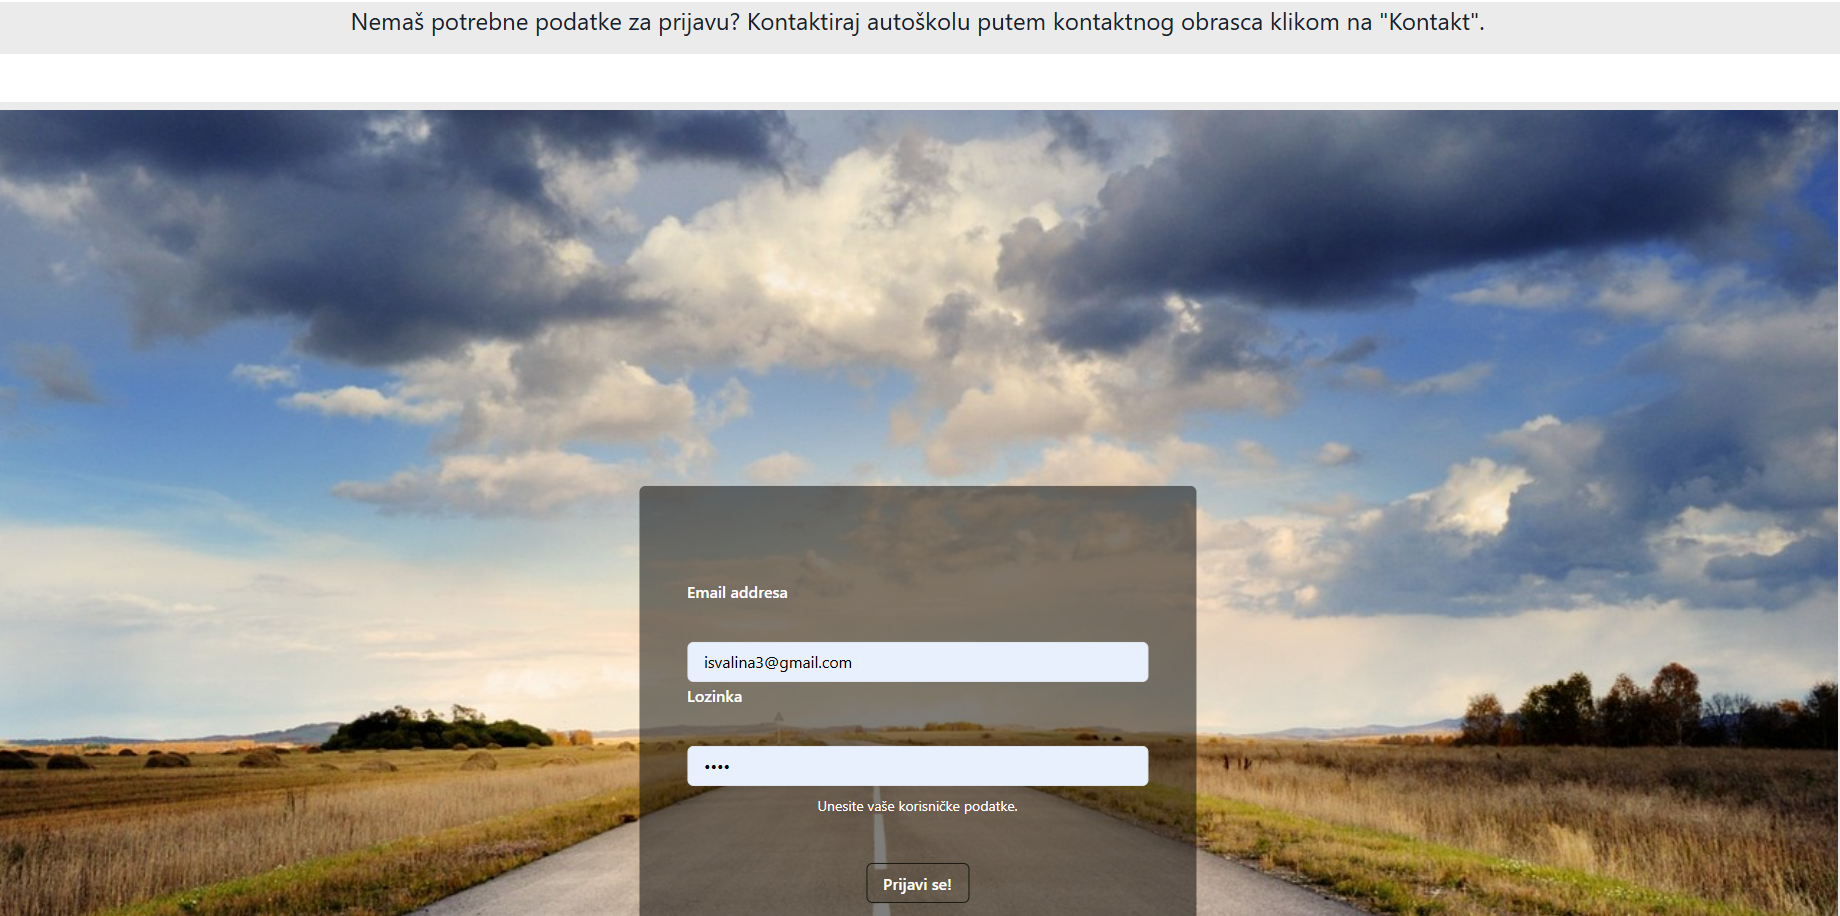
\includegraphics[width=\textwidth]{slike/anoniman2.png} 
					\centering
					\caption{Stranica za prijavu}
					\label{fig:promjene}
				\end{figure}

\noindent Ako korisnik želi dobiti više informacija o autoškoli i aplikaciji, može dabrati opciju "Info" u navigacijskoj traci. Sučelje koje mu se prikazuje je na slici 4.3. i 4.4.

\begin{figure}[H]
					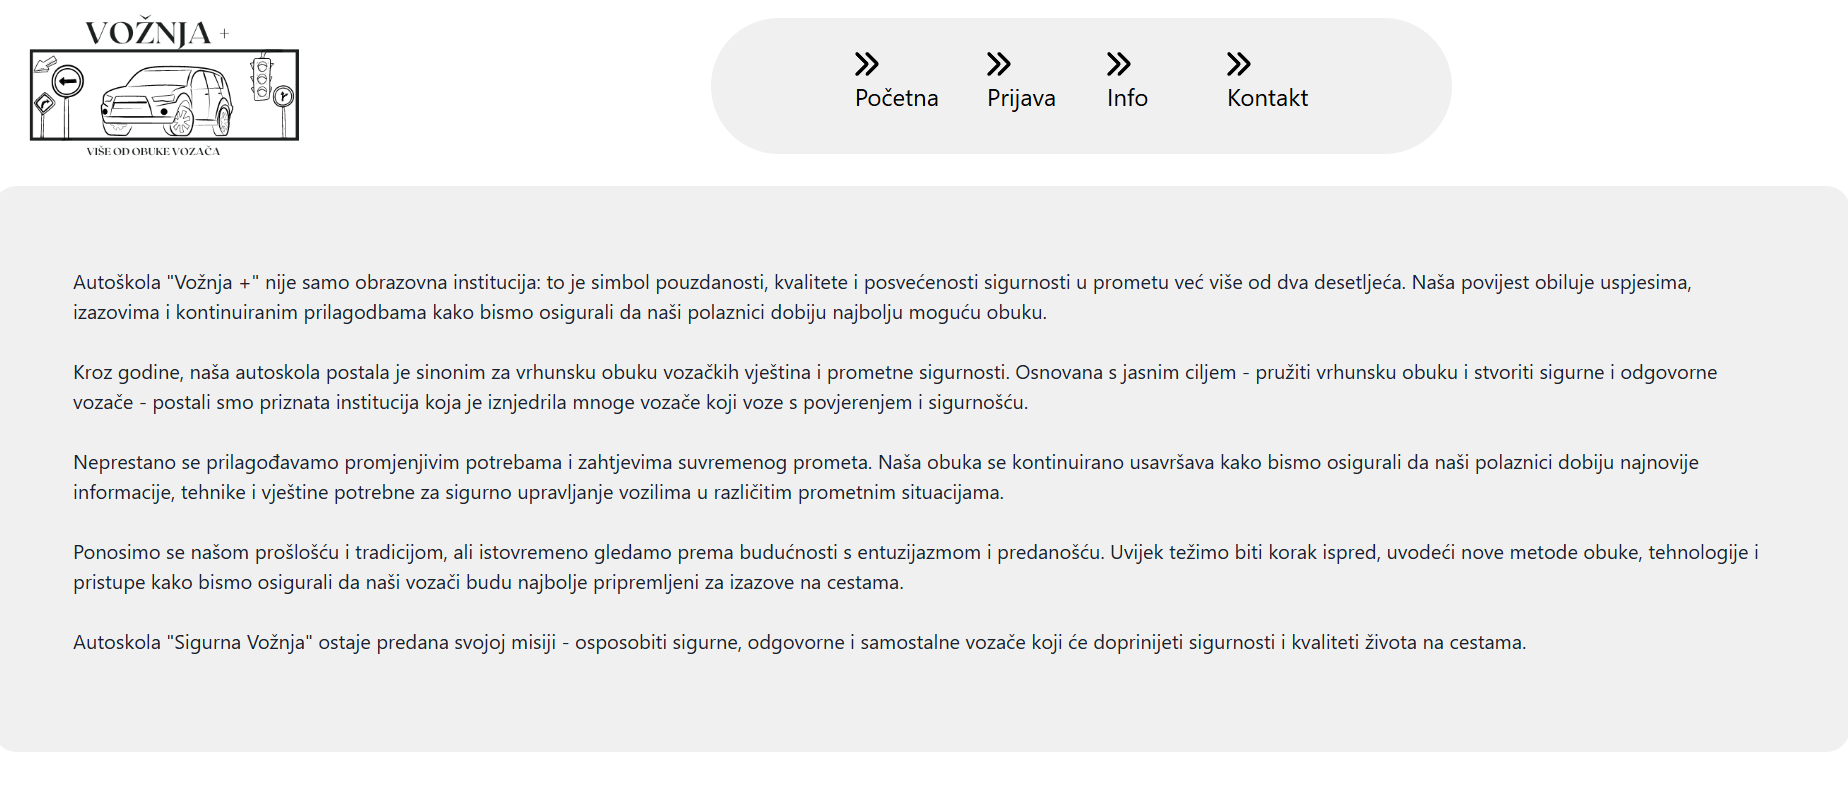
\includegraphics[width=\textwidth]{slike/anoniman3.png} 
					\centering
					\caption{Stranica s dodatnim informacijama}
					\label{fig:promjene}
				\end{figure}

    
\begin{figure}[H]
					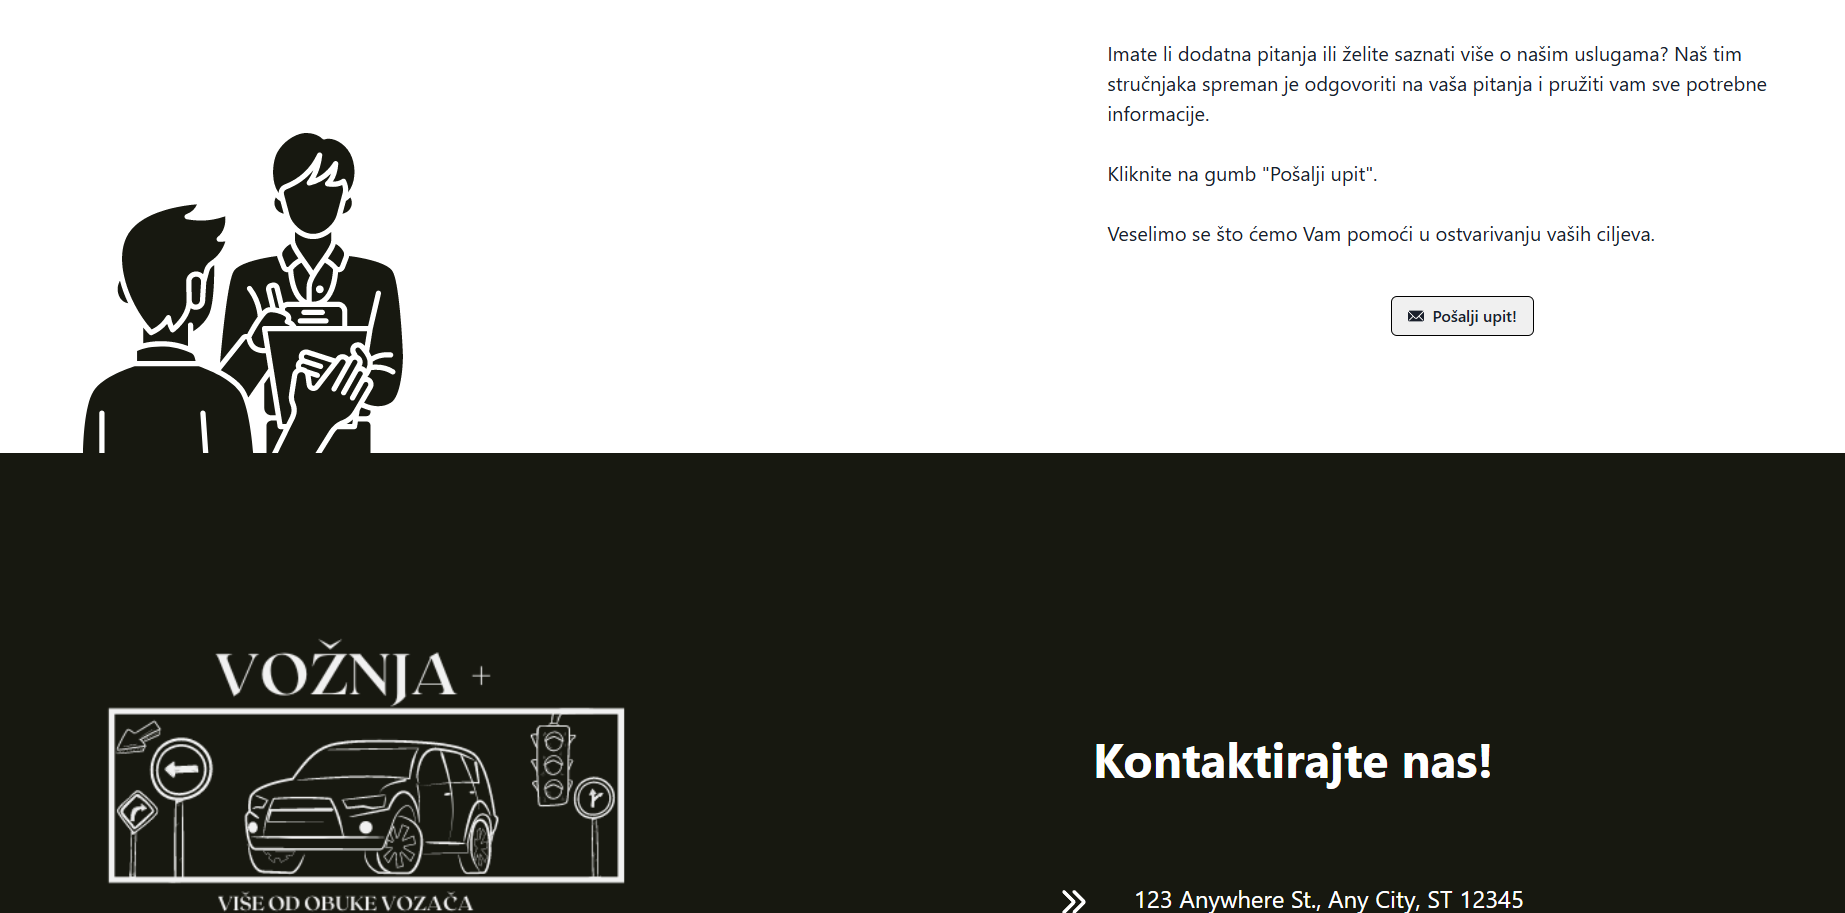
\includegraphics[width=\textwidth]{slike/anoniman4.png} 
					\centering
					\caption{Stranica s dodatnim informacijama}
					\label{fig:promjene}
				\end{figure}

\noindent Za slanje kontaktne forme korisnik odabire opciju "Kontakt" u navigacijskoj traci ili "Pošalji upit" te mu se prikazuje sučelje na slici 4.5.

\begin{figure}[H]
					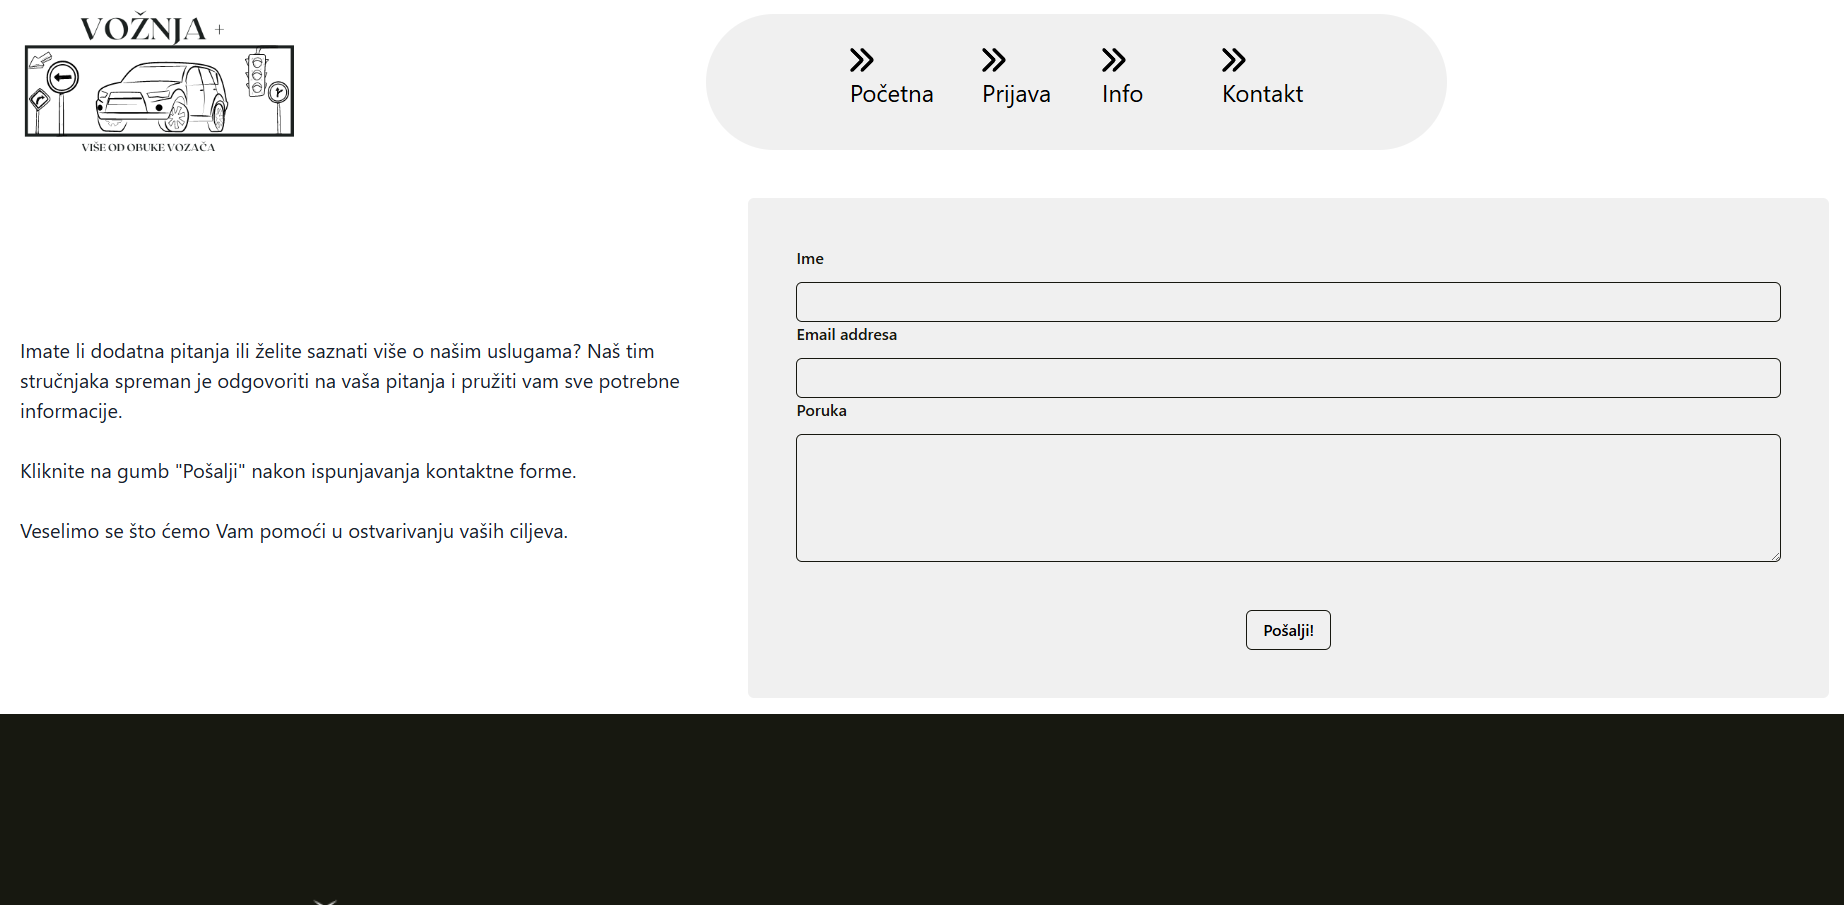
\includegraphics[width=\textwidth]{slike/anoniman5.png} 
					\centering
					\caption{Stranica s kontakt formom}
					\label{fig:promjene}
				\end{figure}


\noindent \textbf{Sučelja polaznika autoškole }\\

\noindent Nakon što se kandidat prijavi u aplikaciju, pored osnovnih, omogućen mu je pristup dodatnim web stranicama. Na slici 4.6. možemo vidjeti kako izgleda stranica s vlastitim korisničkim podacima kojoj može pristupiti svaki autentificiran korisnik.

\begin{figure}[H]
					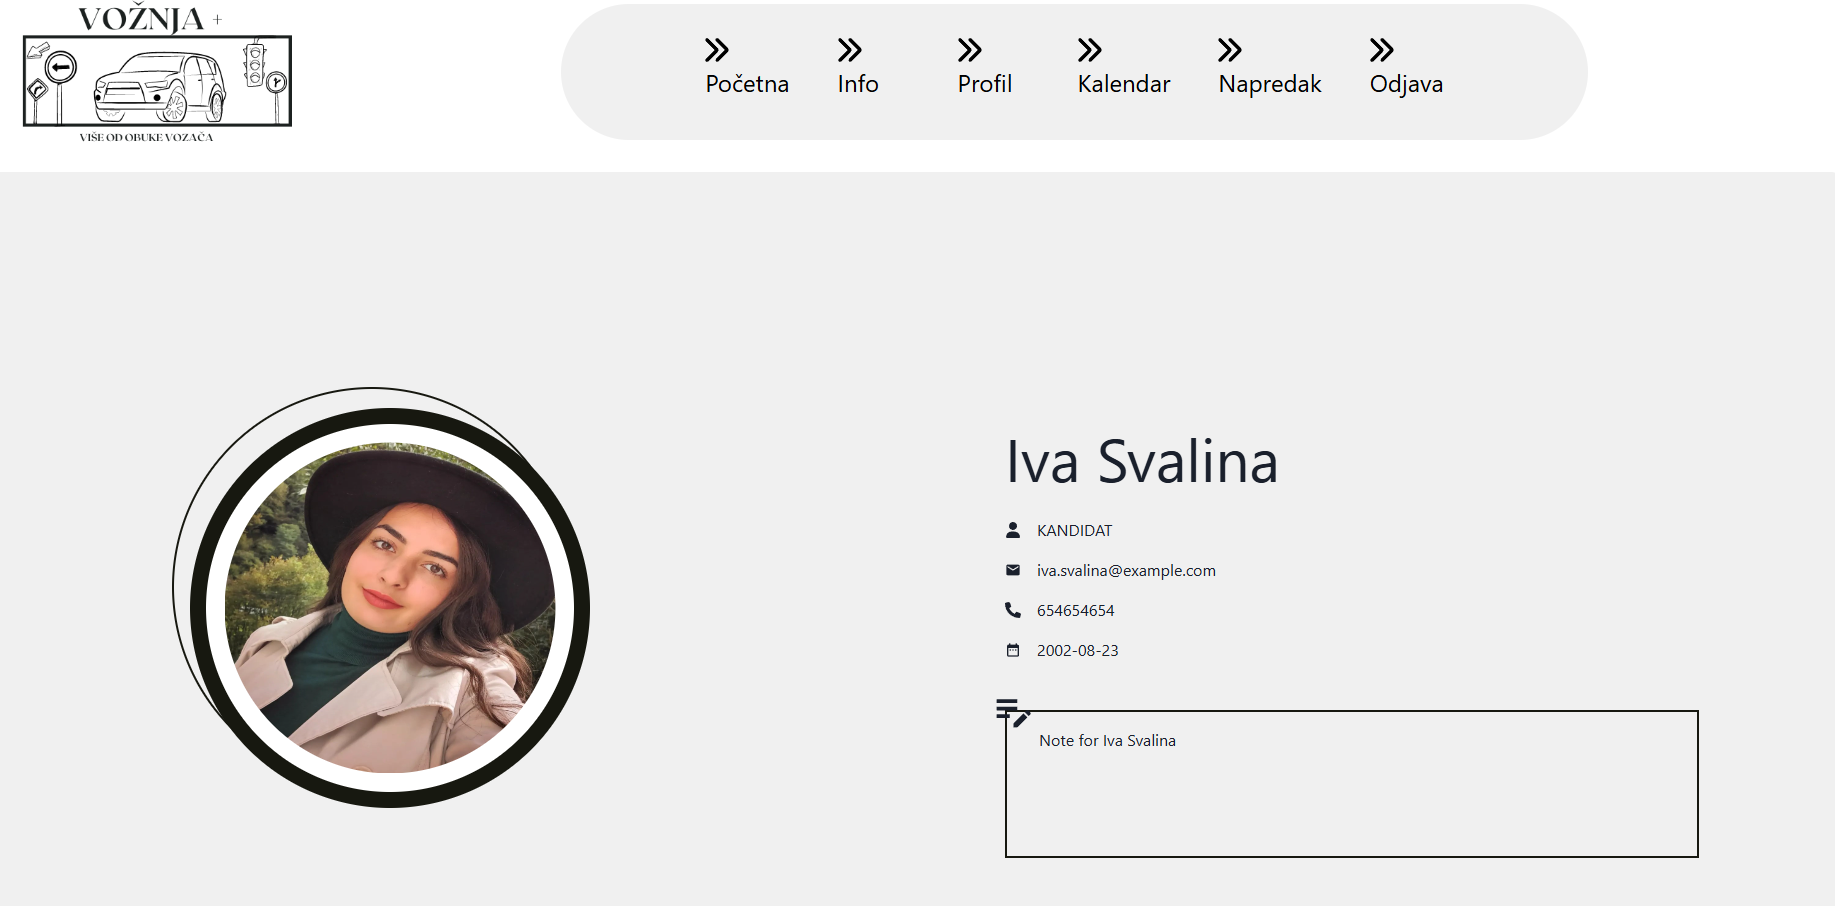
\includegraphics[width=\textwidth]{slike/kandidat1.png} 
					\centering
					\caption{Stranica s kontakt formom}
					\label{fig:promjene}
				\end{figure}

\noindent Odabirom opcija "Kalendar" u navigacijskoj traci korisniku se prikazuje sučelje na slici 4.7. Korisnik događaje u kalendaru može dodavati, uređivati i brisati, što je prikazano na slici 4.8.

\begin{figure}[H]
					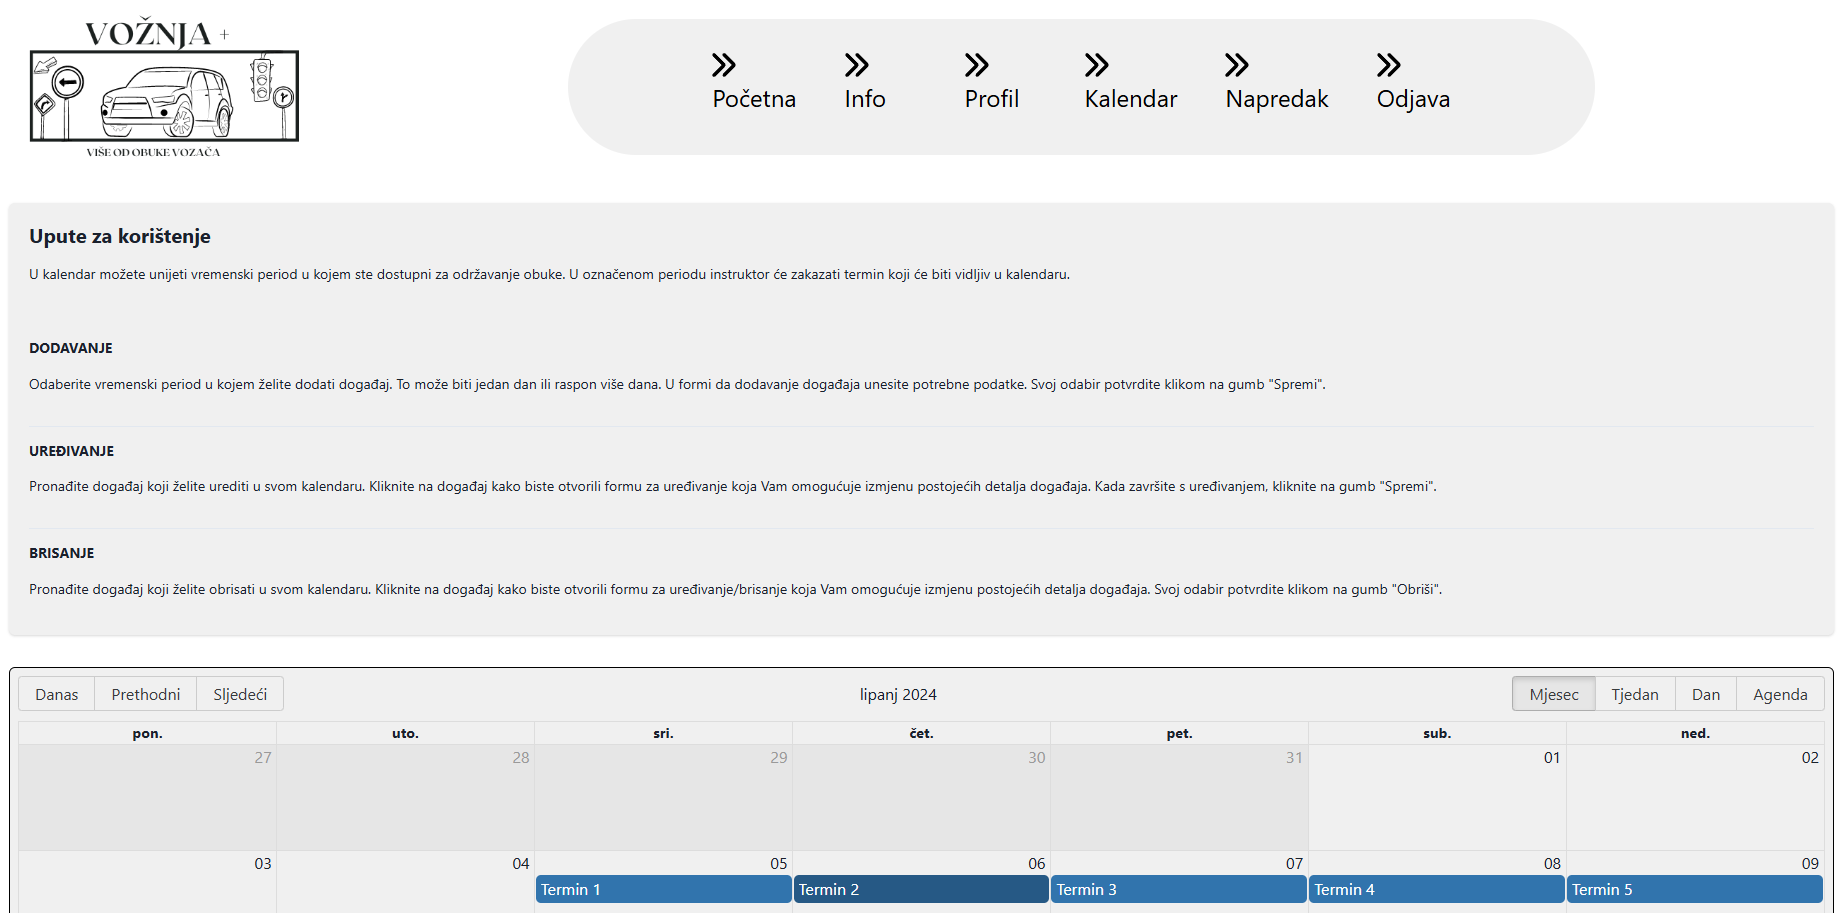
\includegraphics[width=\textwidth]{slike/kandidat2.png} 
					\centering
					\caption{Stranica s kalendarom}
					\label{fig:promjene}
				\end{figure}

    \begin{figure}[H]
					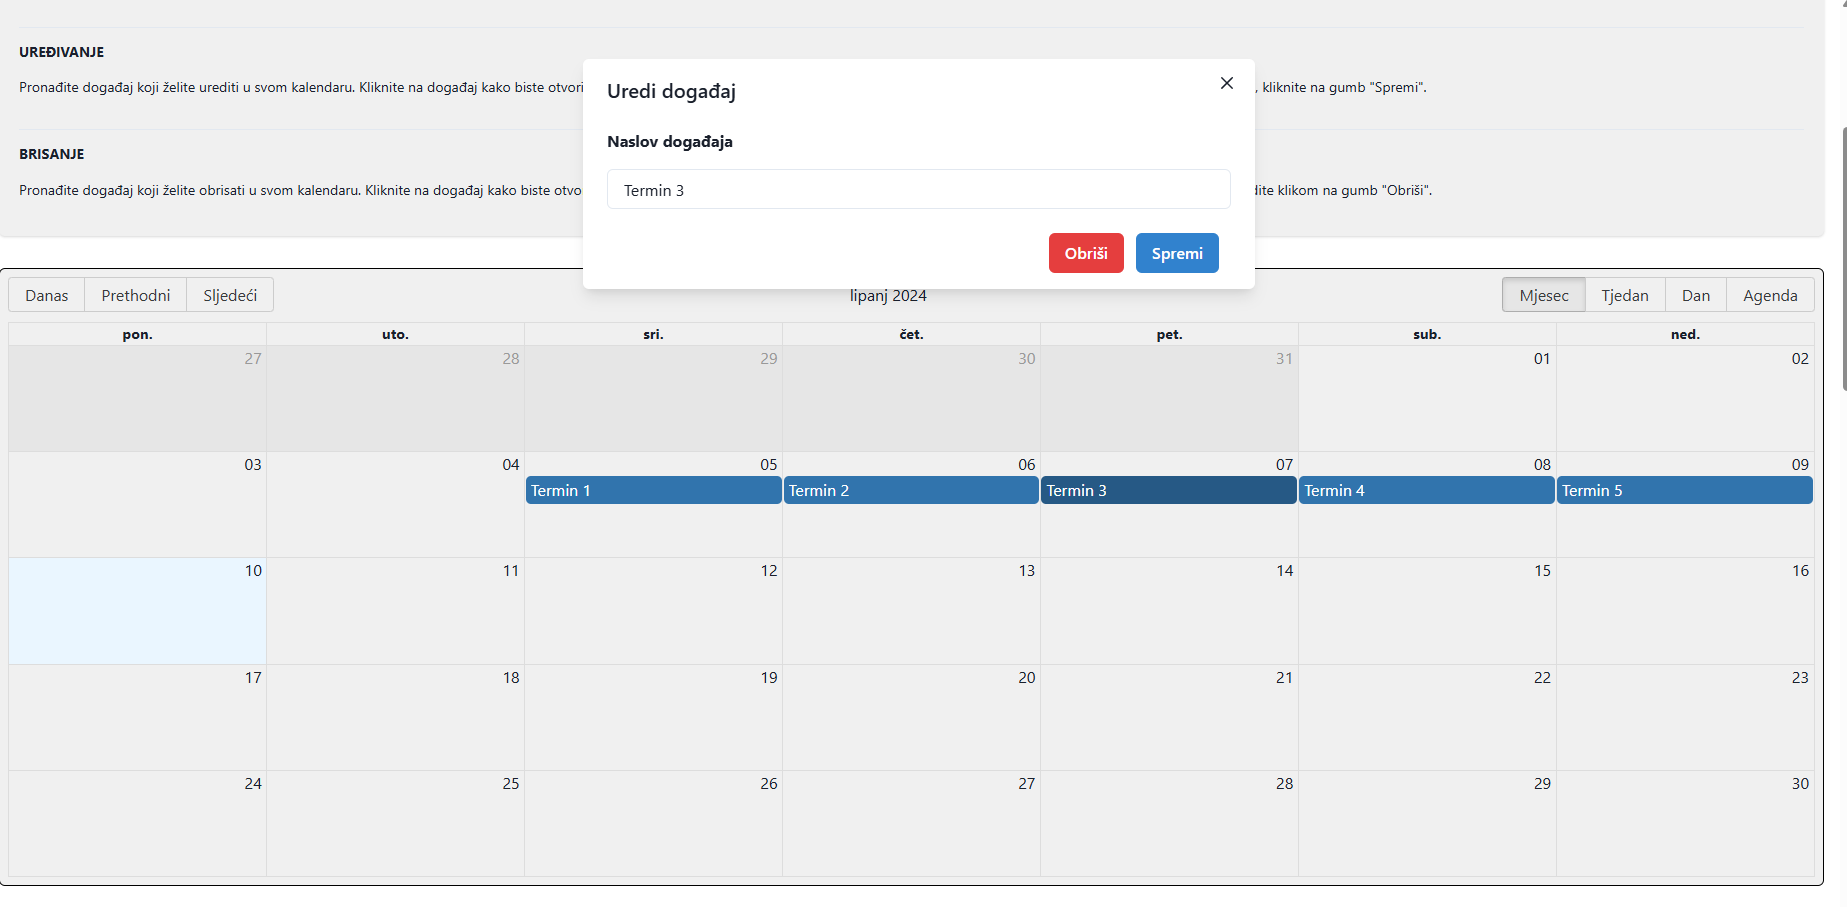
\includegraphics[width=\textwidth]{slike/kandidat3.png} 
					\centering
					\caption{Uređivanje događaja u kalendaru}
					\label{fig:promjene}
				\end{figure}

\noindent Za prikaz stranice napredak na slici 4.9. korisnik odabire opciju "Napredak" u navigacijskoj traci. Svaki predviđeni sat vožnje ima pripadajuću bilješku koja se može vidjeti na slici 4.10.

\begin{figure}[H]
					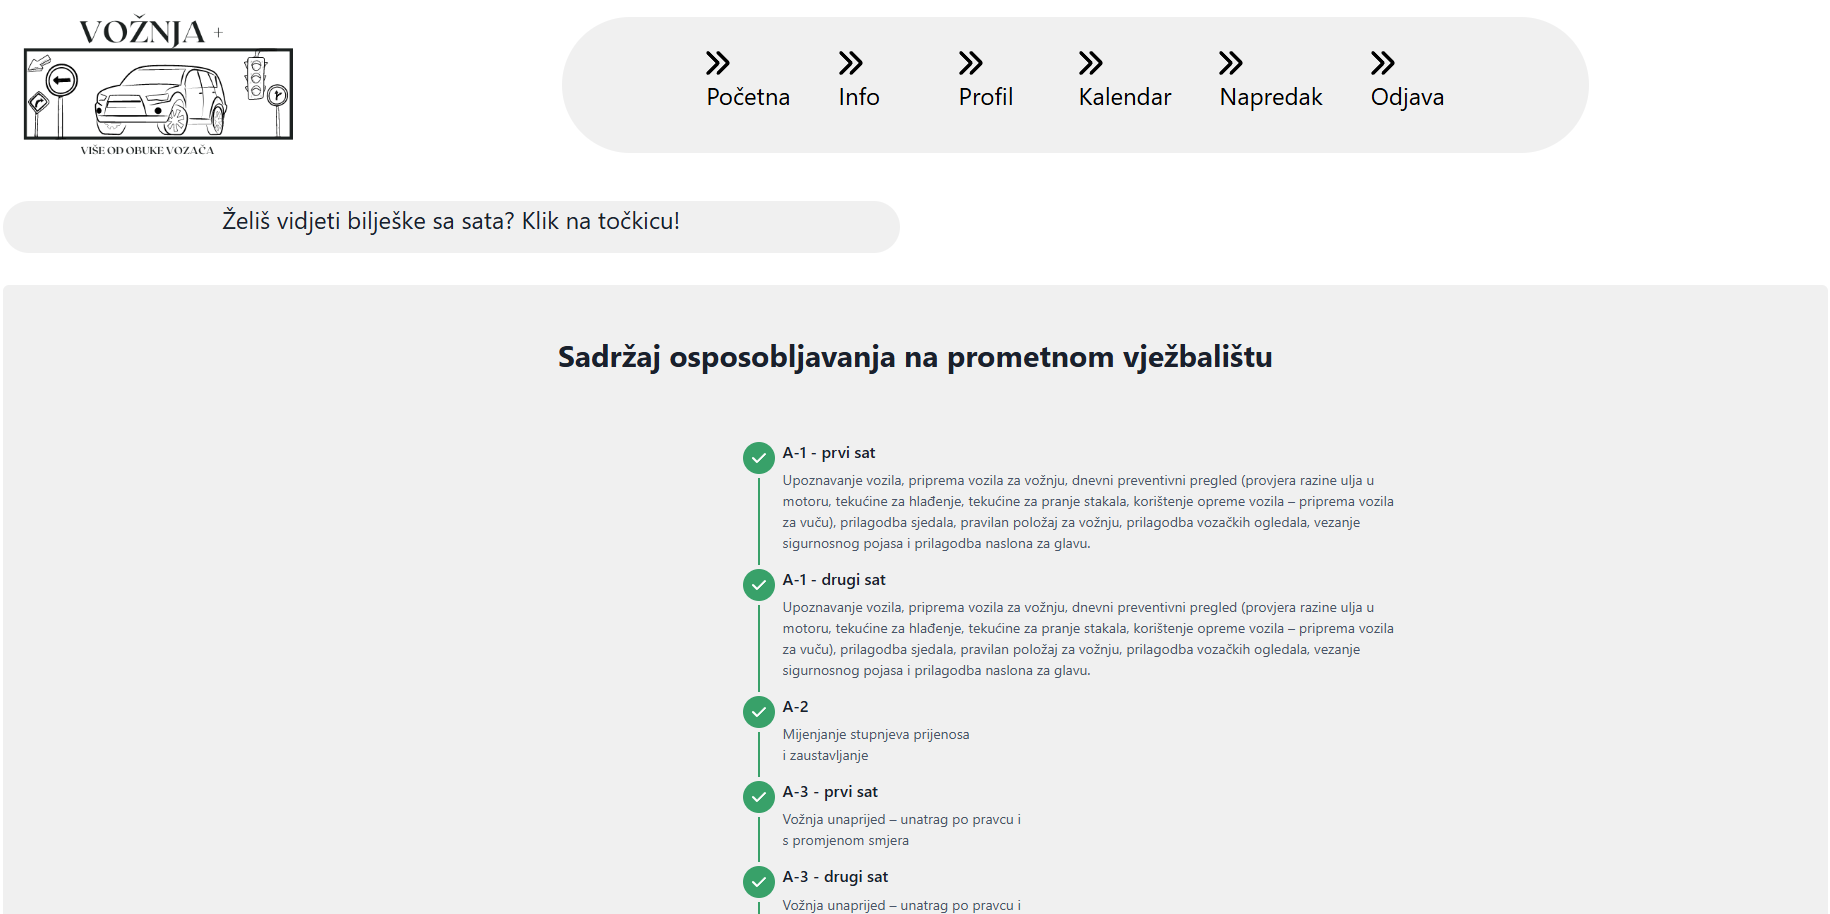
\includegraphics[width=\textwidth]{slike/kandidat4.png} 
					\centering
					\caption{Napredak stranica}
					\label{fig:promjene}
				\end{figure}

    \begin{figure}[H]
					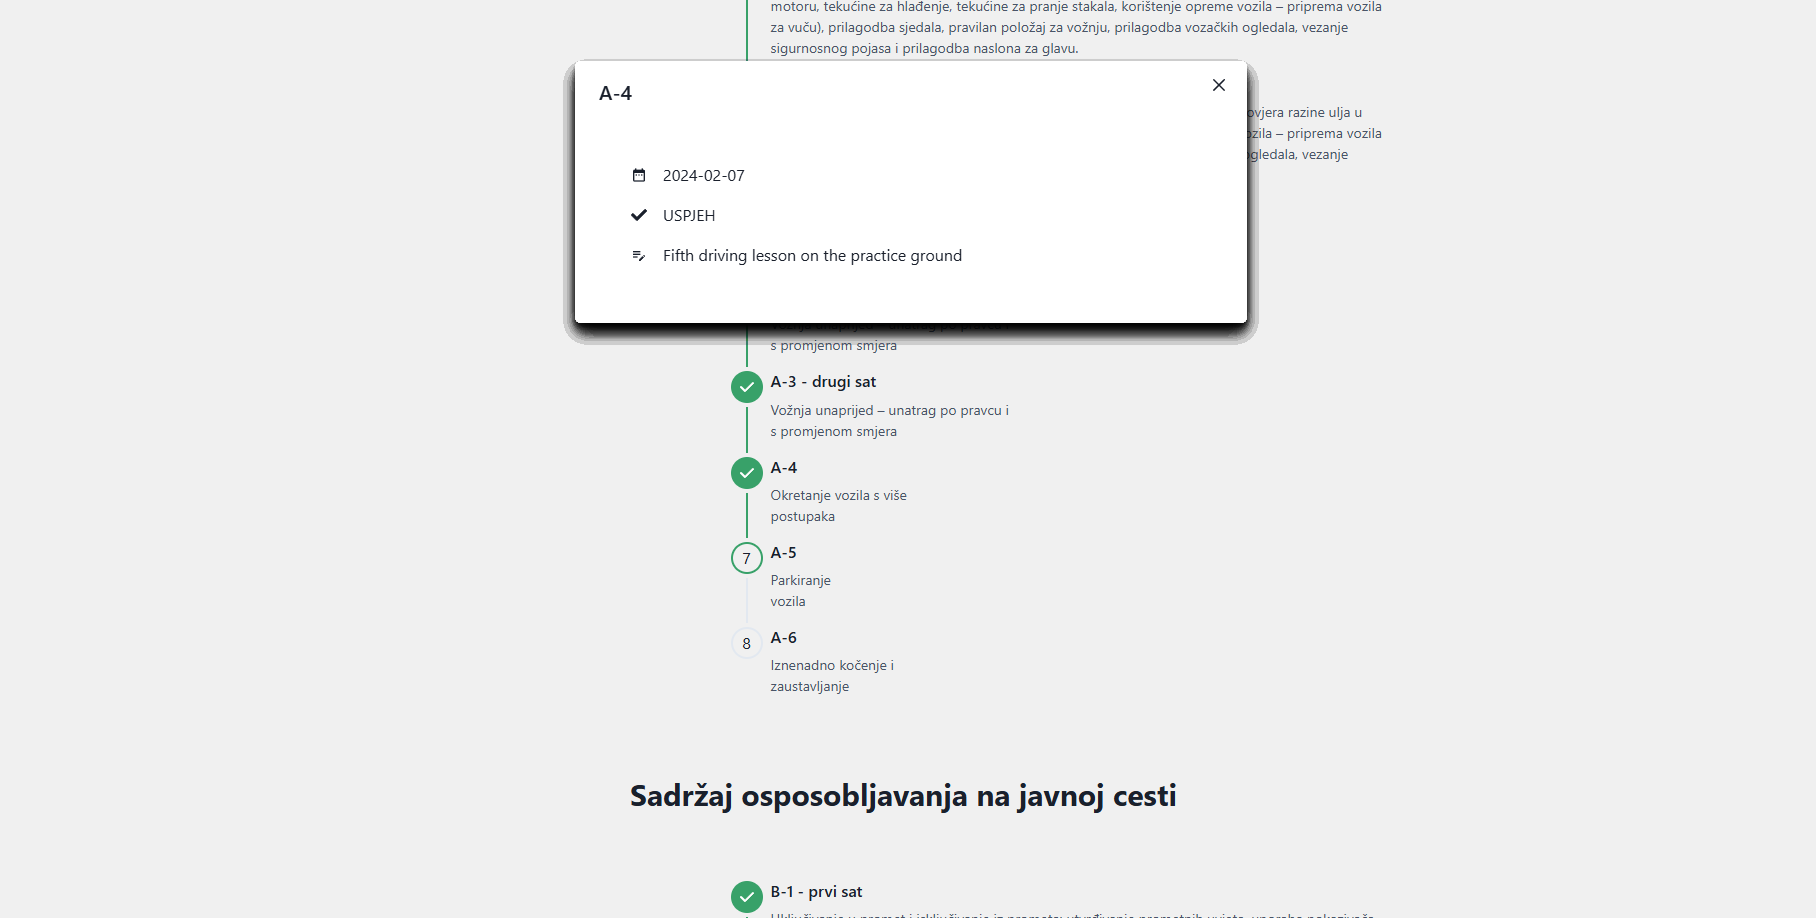
\includegraphics[width=\textwidth]{slike/kandidat5.png} 
					\centering
					\caption{Bilješka za sat}
					\label{fig:promjene}
				\end{figure}

\noindent \textbf{Sučelja instruktora autoškole }\\

\noindent Nakon što se instruktor prijavi u aplikaciju, pored osnovnih, omogućen mu je pristup dodatnim web stranicama. Na slici 4.11. možemo vidjeti kako izgleda stranica sa svim kandidatima kojoj mogu pristupiti instruktori i administratori.

\begin{figure}[H]
					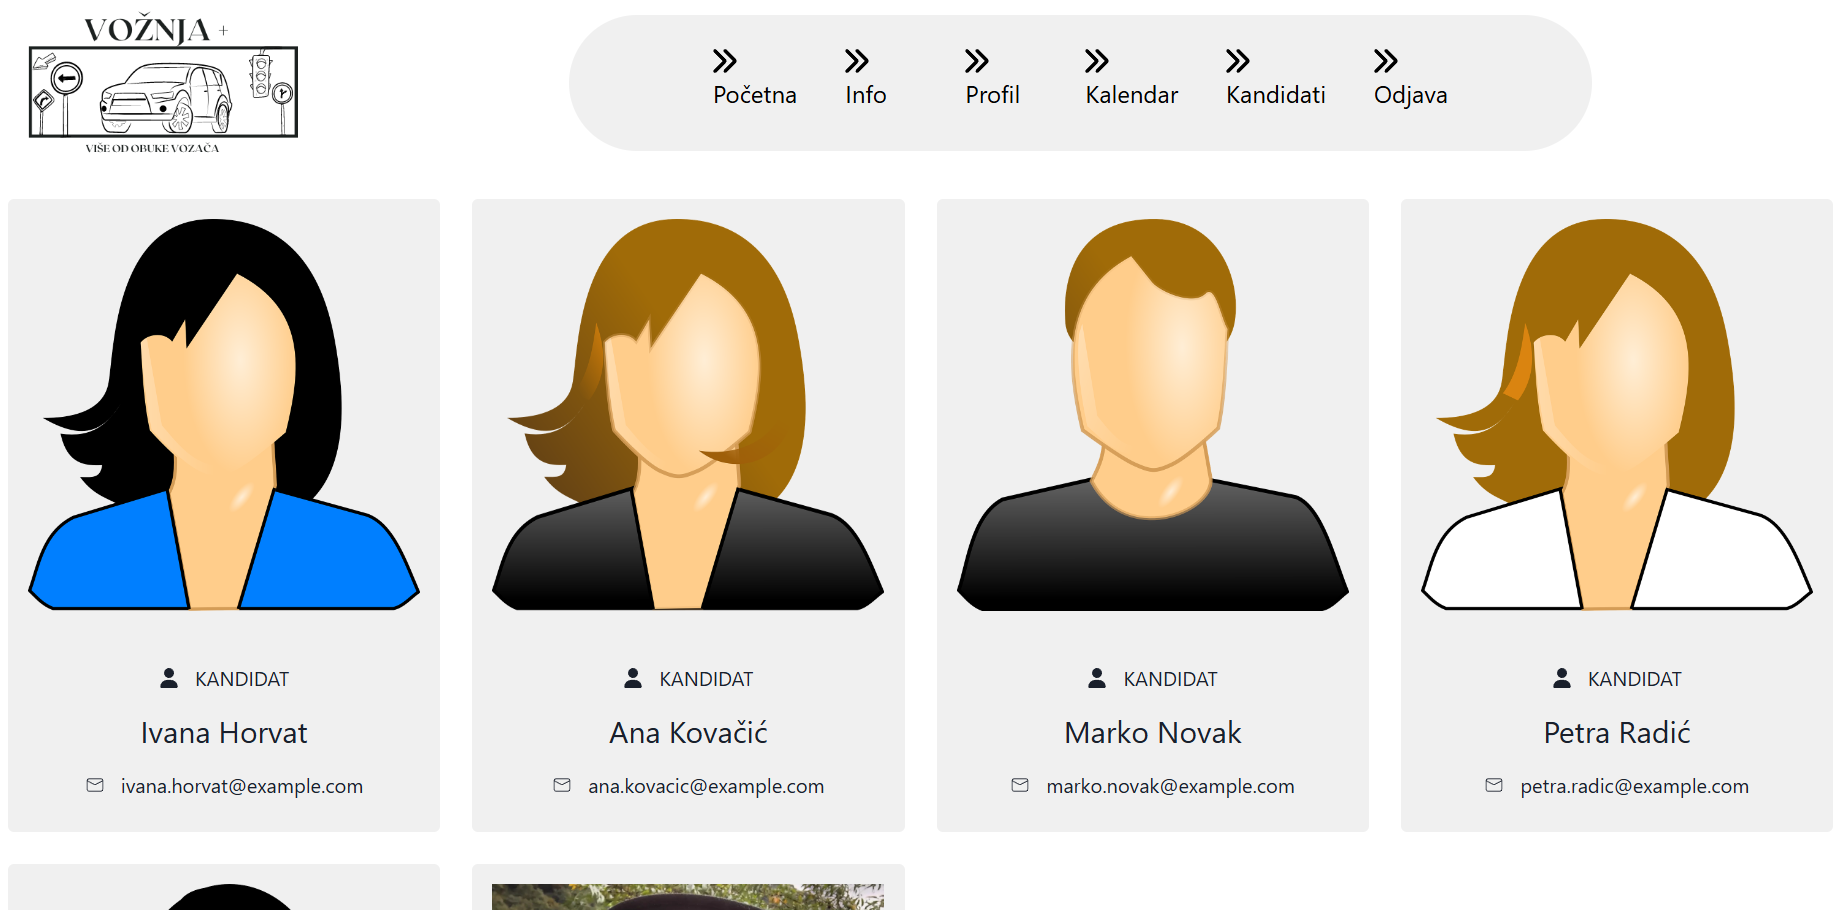
\includegraphics[width=\textwidth]{slike/instruktor1.png} 
					\centering
					\caption{Prikaz svih kandidata}
					\label{fig:promjene}
				\end{figure}

\noindent Nakon odabira na određenog kandidata iz prikaza prikazuje se stranica na slici 4.12. Putem prikazanog sučelja instruktor može pregledati kandidatov kalendar te u njega upisati, urediti ili obrisati termin. Osim toga, instruktor unosi bilješke za održani sat putem sučelja prikazanog na slici 4.13.

\begin{figure}[H]
					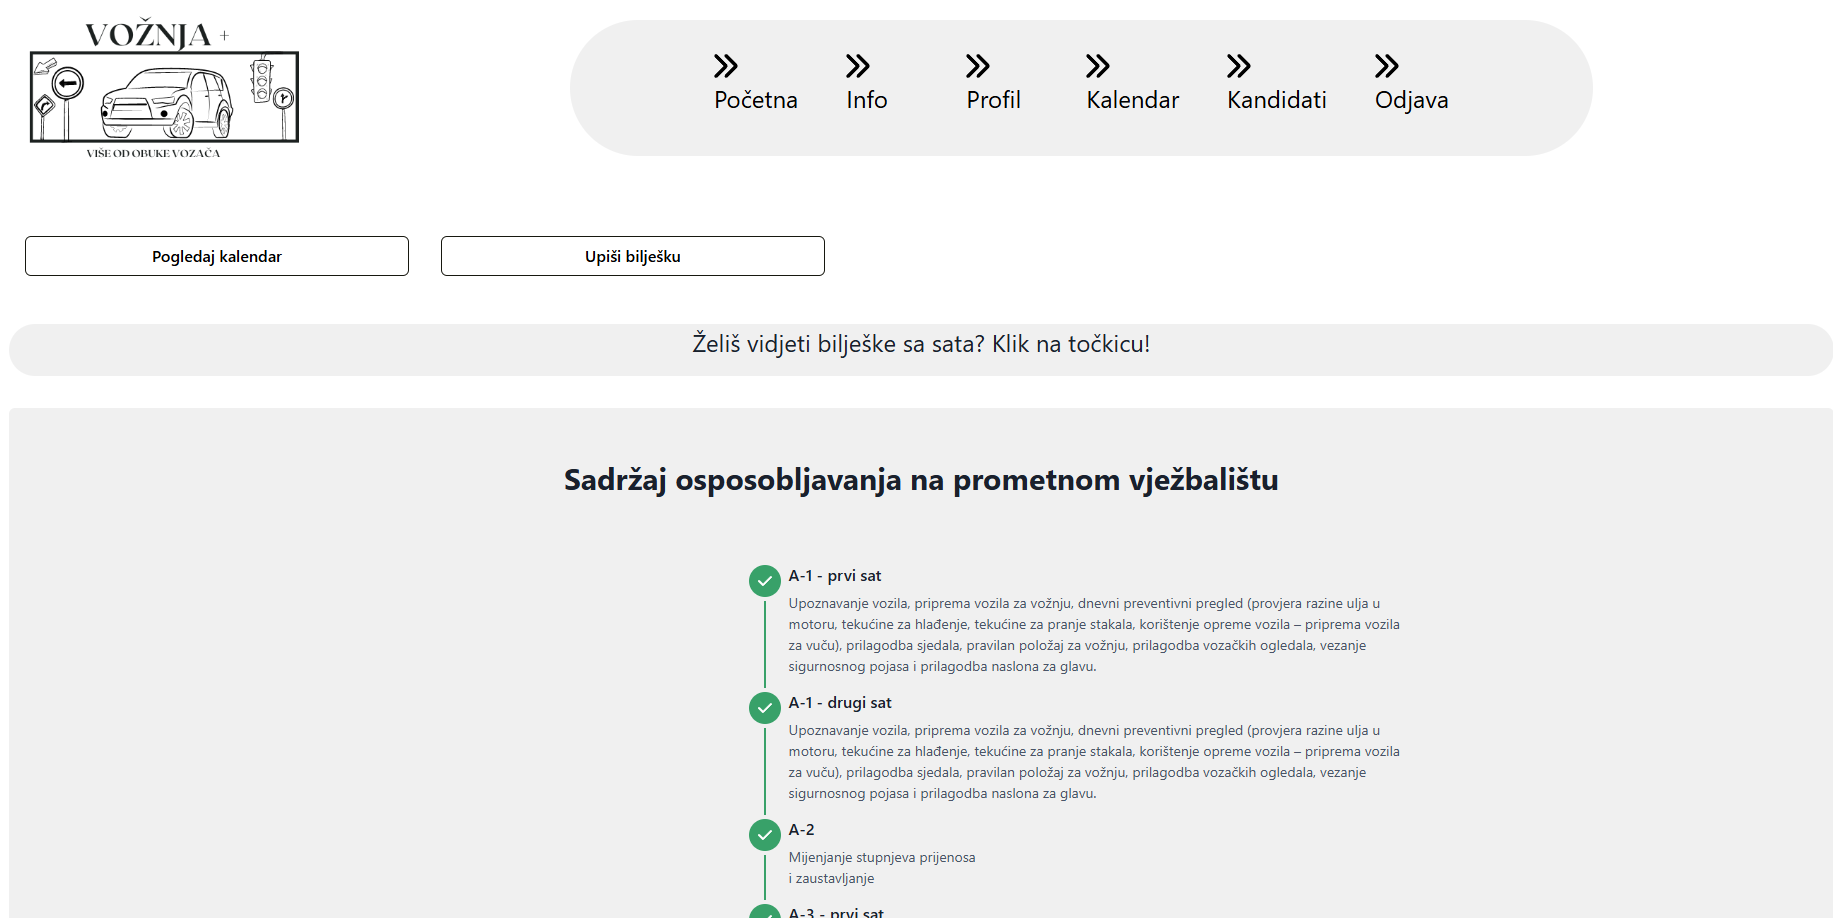
\includegraphics[width=\textwidth]{slike/instruktor2.png} 
					\centering
					\caption{Prikaz stranice za napredak}
					\label{fig:promjene}
				\end{figure}
\begin{figure}[H]
					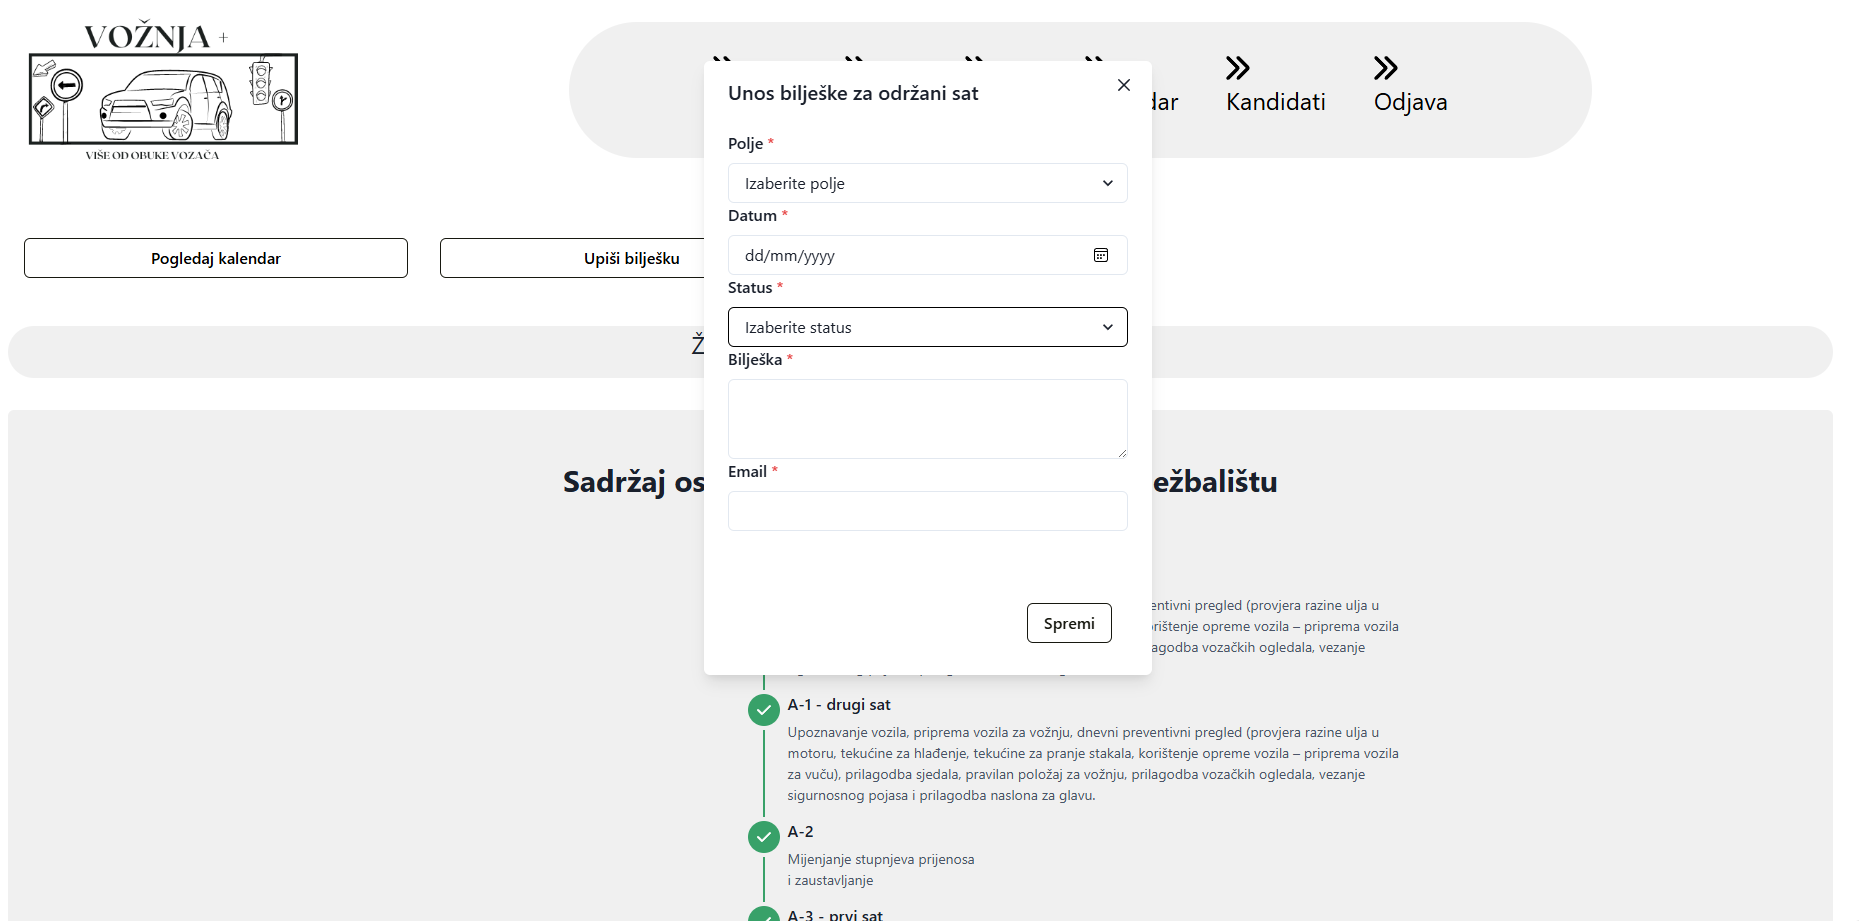
\includegraphics[width=\textwidth]{slike/instruktor3.png} 
					\centering
					\caption{Unos bilješke sa sata}
					\label{fig:promjene}
				\end{figure}

\noindent \textbf{Sučelja administratora autoškole }\\

\noindent Nakon što se administrator prijavi u aplikaciju, pored osnovnih, omogućen mu je pristup dodatnim web stranicama. Na slici 4.14. možemo vidjeti kako izgleda stranica koja prikazuje sve instruktore. Spomenutoj stranici može pristupiti samo administrator. Klikom na određenog instruktora prikazuje se stranica s kalendarom odabranog korisnika.

\begin{figure}[H]
					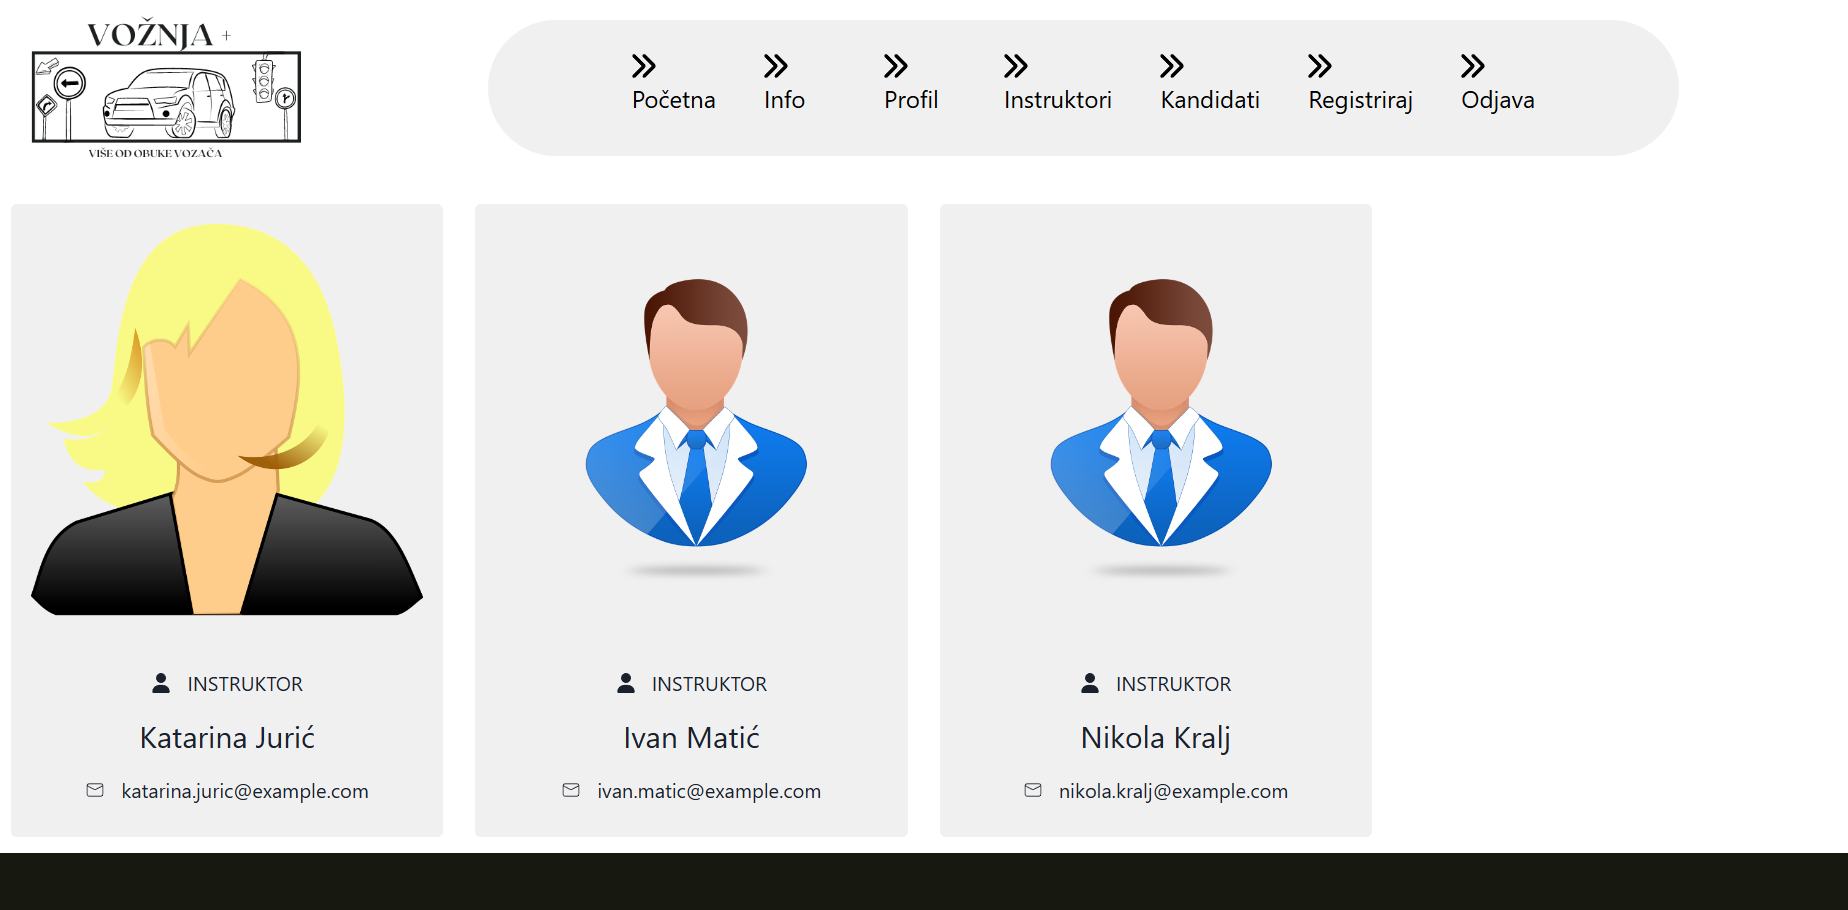
\includegraphics[width=\textwidth]{slike/admin1.png} 
					\centering
					\caption{Prikaz instruktora}
					\label{fig:promjene}
				\end{figure}

\noindent Na kraju, na slikama 4.15 i 4.16. možemo vidjeti prikaz forme za registraciju novih korisnika kojoj također može pristupiti isključivo korisnik s ulogom administratora. Na slici 4.16 vidi se i univerzalno podnožje svake stranice na kojem se mogu naći kontakt podaci.

\begin{figure}[H]
					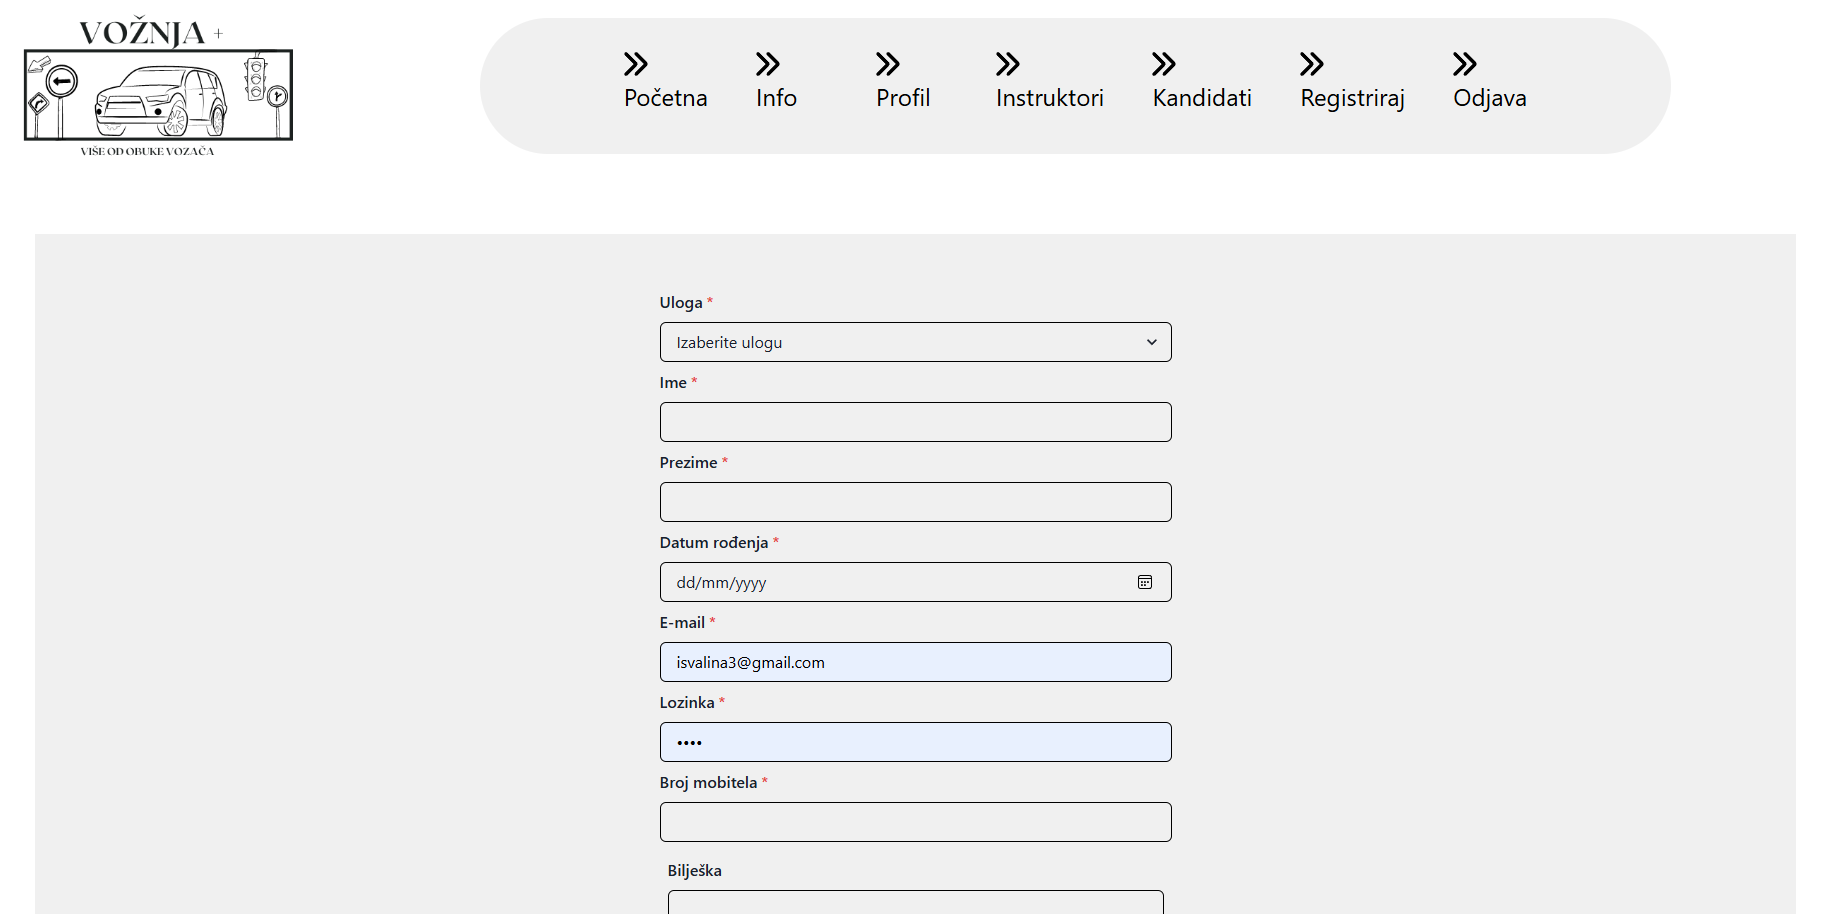
\includegraphics[width=\textwidth]{slike/admin2.png} 
					\centering
					\caption{Registracija novog korisnika}
					\label{fig:promjene}
				\end{figure}

    
\begin{figure}[H]
					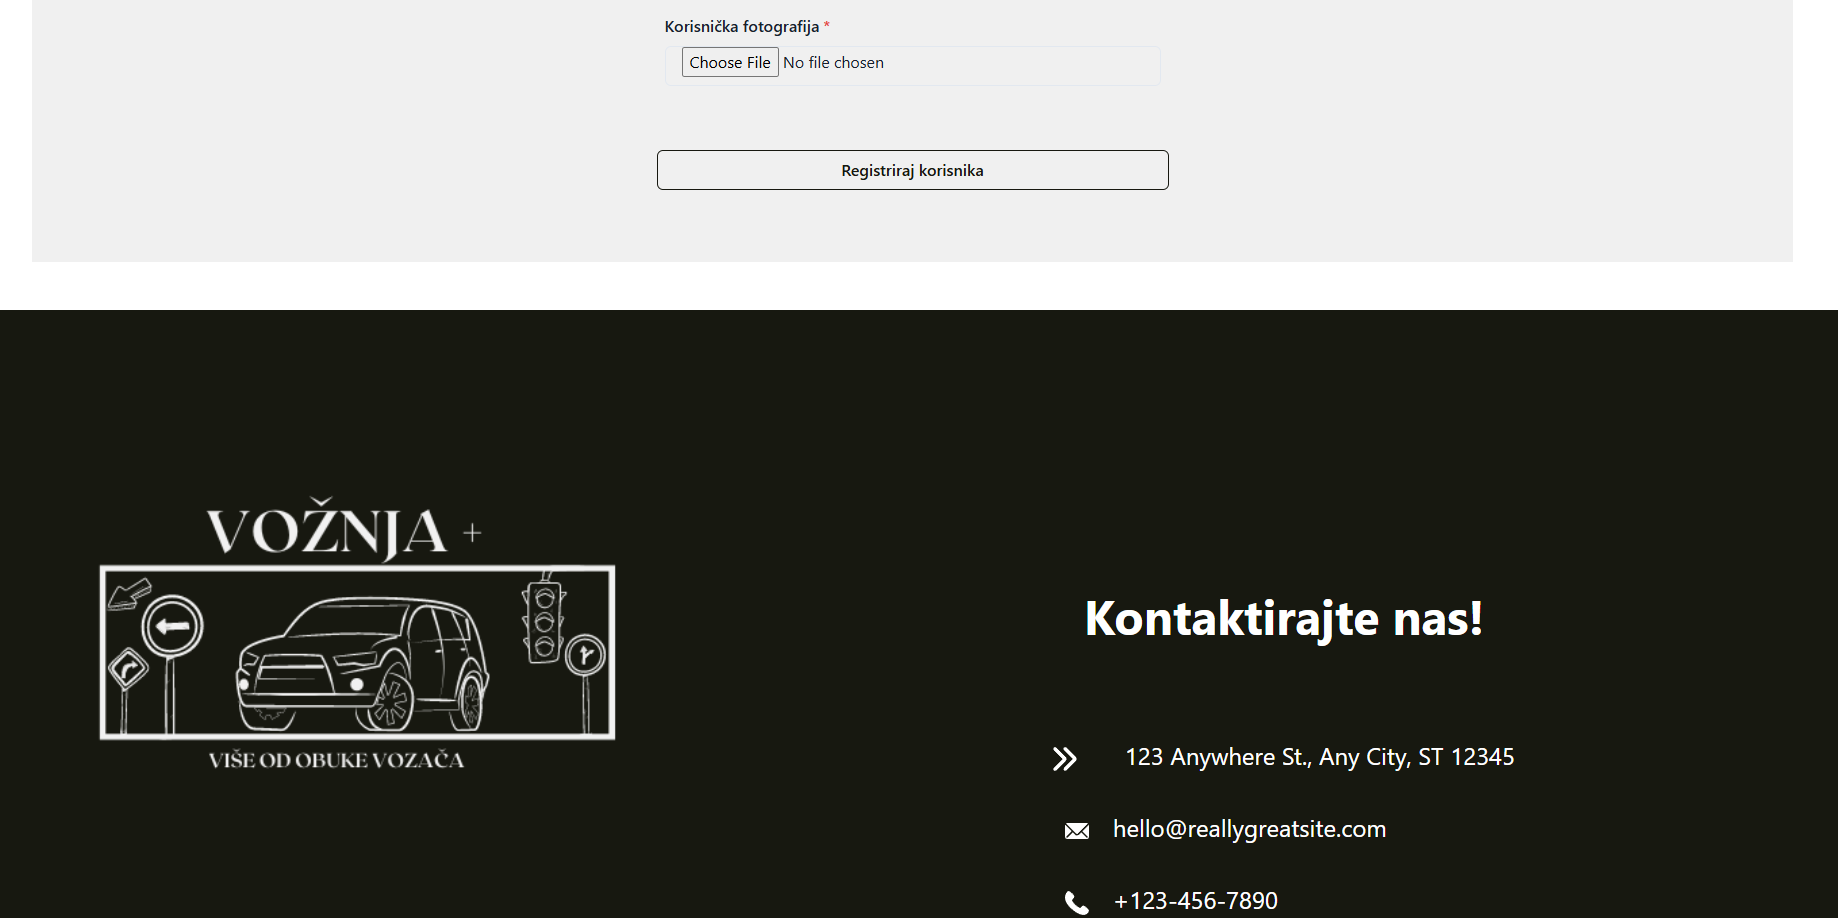
\includegraphics[width=\textwidth]{slike/admin3.png} 
					\centering
					\caption{Registracija novog korisnika i kontakt podaci}
					\label{fig:promjene}
				\end{figure}